\documentclass[a4paper,12pt]{article}

%% Language and font encodings
\usepackage[T1]{fontenc}
\usepackage[polish]{babel}
\usepackage[utf8]{inputenc}
\usepackage{lmodern}
\selectlanguage{polish}

%% Sets page size and margins
%\usepackage[a4paper,top=2cm,bottom=2cm,left=2cm,right=4cm,asymmetric]{geometry}
\usepackage{geometry}


%% Useful packages
\usepackage[fleqn]{amsmath}%[fleqn]
\usepackage{xfrac} %\sfrac{}{}

\usepackage{titlesec}%titles
\titlelabel{\thetitle.\quad}
\let\savenumberline\numberline
\def\numberline#1{\savenumberline{#1.}}
\usepackage{etoolbox}%dots in TOC
\makeatletter
\patchcmd{\l@section}
{\hfil}
{\leaders\hbox{\normalfont$\m@th\mkern \@dotsep mu\hbox{.}\mkern \@dotsep mu$}\hfill}
{}{}
\makeatother

\usepackage{caption,graphicx}
\usepackage{float}
\usepackage{sidecap}
\usepackage[colorinlistoftodos]{todonotes}
\usepackage[colorlinks=true, allcolors=blue]{hyperref}

\usepackage{tikz}
\usepackage{tikz-qtree}
\usetikzlibrary{trees}
\usetikzlibrary{arrows,positioning,shapes,fit,calc,decorations.pathreplacing}
\usetikzlibrary{graphs}
\usetikzlibrary{graphs.standard}
\usepackage{forest}
\usepackage{tikzscale}
\usepackage{pgfgantt} %Diagramy gantta http://bay.uchicago.edu/CTAN/graphics/pgf/contrib/pgfgantt/pgfgantt.pdf
\usepackage{pgf}
\usepackage{caption}

\usepackage{fancybox}
\usepackage{listings}

\usepackage[colorinlistoftodos]{todonotes} %http://mirror.unl.edu/ctan/macros/latex/contrib/todonotes/todonotes.pdf

\usepackage{array,longtable}

\newcommand\floor[1]{\lfloor#1\rfloor} %PODŁOGA -> \floor
\newcommand\ceil[1]{\lceil#1\rceil} %SUFIT -> \ceil

\usepackage{fancyhdr}
\pagestyle{fancy}
\rhead{\thepage}
\lhead{\leftmark}
\rfoot{\thepage}
\lfoot{\rightmark}

%http://tex.stackexchange.com/questions/64170/which-package-to-use-for-writing-algorithms
\usepackage{algorithm}% http://ctan.org/pkg/algorithms
\usepackage{algpseudocode}% http://ctan.org/pkg/algorithmicx
\newcommand{\var}[1]{{\ttfamily#1}}% variable

\algnewcommand\algorithmicforeach{\textbf{for each}} %Algorithm foreach
\algdef{S}[FOR]{ForEach}[1]{\algorithmicforeach\ #1\ \algorithmicdo}

\usepackage{amsthm}
\usepackage[inline]{enumitem} %enumerations
\usepackage{multicol}

\theoremstyle{definition}%~ %%% <-  Note that space!
\newtheorem{lemma}{Lemat} %\begin{lemma} ... \end{lemma} LEMAT(?)
\newtheorem{remark}{Wniosek}%\begin{remark} ... \end{remark} WNIOSEK 
%\newtheorem*{remark*}{Wniosek}%\begin{remark} ... \end{remark} WNIOSEK bez liczby
\newtheorem{theorem}{Twierdzenie}%\begin{theorem} ... \end{theorem}
\newtheorem{fact}{Fakt} %\begin{fact} ... \end{fact}
\newtheorem*{fact*}{Fakt} %\begin{fact*} ... \end{fact*} Fakt
\newtheorem*{observation*}{Obserwacja}

\newtheorem{example}{Przykład}
\newtheorem*{example*}{Przykład} %\begin{example} ... \end{example}
\theoremstyle{definition}
\newtheorem{definition}{Definicja}%\begin{definition}{} ... \end{definition}
%\newtheorem*{definition*}{Definicja}
%\newtheorem*{hipoterm*}{Hipoteza}%\begin{hipoterm*}[] ... \end{hipoterm*}
\newtheorem{hipoterm}{Hipoteza}%\begin{hipoterm*}[] ... \end{hipoterm*}
\theoremstyle{problem}
\newtheorem{problem}{Problem}%\begin{problem}{} ... \end{problem}
\newtheorem*{problem*}{Problem}

\let\originalforall=\forall%FORALL
\renewcommand{\forall}{\mathop{\vcenter{\hbox{\Large$\originalforall$}}}}
\let\originalexists=\exists%EXISTS
\renewcommand{\exists}{\mathop{\vcenter{\hbox{\Large$\originalexists$}}}}

\usepackage{cancel} %skreślenie równania \xcancel{...} \cancel{} lub \bcancel{}

\usepackage{amsfonts}

\usepackage{comment}

\usepackage{xcolor,colortbl}
\usepackage{multirow}

%\usepackage{wrapfig} %wrap text around figure

\usepackage{pdfpages}%\includepdf{file}

\usepackage{etoolbox}
\let\bbordermatrix\bordermatrix
\patchcmd{\bbordermatrix}{8.75}{4.75}{}{}
\patchcmd{\bbordermatrix}{\left(}{\left[}{}{}
\patchcmd{\bbordermatrix}{\right)}{\right]}{}{}
%\bbordermatrix{}

\allowdisplaybreaks

\title{Struktury Dyskretne - Notatki}
\author{Piotr Parysek\\
\href{mailto:piotr.parysek@outlook.com}{piotr.parysek@outlook.com} }
\date{\today}

\begin{document}
\maketitle

\tableofcontents
\section[Wykład 2: 2-III-2017 - Temat: kody Eulera i Cykle Hamiltona]{Temat: kody Eulera i Cykle Hamiltona}
\begin{figure}[H]
\centering
\begin{minipage}{.75\textwidth}
\centering
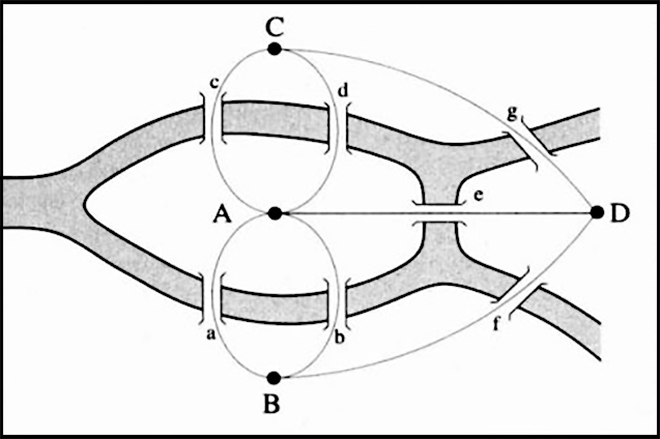
\includegraphics[width=0.9\textwidth]{img/bridge}
\caption[Problem Eulera z przedstawieniem mostów]{Problem Eulera z przedstawieniem mostów\footnotemark .}
\label{fig:eulerproblem}
\footnotetext{Pobrane ze strony: \url{https://physics.weber.edu/carroll/honors/konigsberg.htm}}
\end{minipage}%
\begin{minipage}{.2\textwidth}
\begin{tikzpicture}[shorten >=1pt, auto, node distance=3cm, ultra thick,main node/.style={circle,draw,minimum size=.4cm,inner sep=0pt]}]%fill=black,
\begin{scope}[every node/.style={font=\sffamily\Large\bfseries}]
\node[main node] (v1) at (2,0) {D};
\node[main node] (v2) at (0,0) {A};
\node[main node] (v3) at (1,1) {C};
\node[main node] (v4) at (1,-1) {B};
\end{scope}
\begin{scope}
\draw  (v1) edge node{} (v2);
\draw  (v1) edge node{} (v3);
\draw  (v1) edge node{} (v4);
\draw  (v2) edge[bend right] node{} (v3);
\draw  (v2) edge[bend left] node{} (v3);
\draw  (v2) edge[bend right] node{} (v4);
\draw  (v2) edge[bend left] node{} (v4);
\end{scope}
\end{tikzpicture}
\caption{Przedstawienie grafowe.}
\label{fig:eulerproblemgraf}
\end{minipage}
\end{figure}

\begin{problem*}[Eulera]~ %%% <-  Note that space!
Czy mogę iść na spacer przechodząc przez każdy most tylko RAZ?
Przedstawienie mostów zaprezentowane na rysunku \ref{fig:eulerproblem} lub \ref{fig:eulerproblemgraf}.
\end{problem*}~ %%% <-  Note that space!
\begin{definition}[Graf prosty]~ %%% <-  Note that space!
Grafem prostym nazywamy graf \textbf{NIE} posiadający pętli własnych i krawędzi wielokrotnych (multikrawędzi). 
\end{definition}
\begin{definition}[Multigraf]~ %%% <-  Note that space!
Graf posiadający multikrawędzie.
\end{definition}
\begin{definition}[Graf spójny]~ %%% <-  Note that space!
Graf posiadający jedną składową.
\end{definition}
\begin{definition}[Graf niespójny]~ %%% <-  Note that space!
Graf posiadający kilka składowych.
\end{definition}
\begin{definition}[Obchód Eulera]~ %%% <-  Note that space!
,,spacer'' po grafie, w którym wychodząc z danego wierzchołka wracamy do niego przechodząc przez \textbf{KAŻDĄ} krawędź dokładnie \textbf{RAZ}.
\end{definition}
\begin{theorem}[Euler]\label{the:euler}~ %%% <-  Note that space!
Niepusty graf ma obchód Eulera (jest Eulerowski) wtedy i tylko  wtedy, gdy nie posiada wierzchołków stopnia nieparzystego
\end{theorem}
\begin{definition}[Szlak Eulera]~ %%% <-  Note that space!
rodzaj obchodu Eulera w którym ,,przechodzi'' się przez wszystkie krawędzie ale nie kończy się w wierzchołku którym się zaczęło.
\end{definition}
\begin{remark}
Graf spójny ma szlak Eulera wtedy i tylko  wtedy, gdy ma co najwyżej dwa wierzchołki stopnia nieparzystego.
\end{remark}
\begin{definition}[Krawędź cięcia]~ %%% <-  Note that space!
Krawędź $e\in E(G)$ nazywamy \textbf{krawędzią cięcia}, gdy usunięcie krawędzi z grafu $G$ powoduje zwiększenie liczby składowych.
\end{definition}
\begin{example*}
Przykład grafu:
\begin{figure}[H]
\centering
\begin{tikzpicture}[shorten >=1pt, auto, node distance=3cm, ultra thick,main node/.style={circle,draw,minimum size=.4cm,inner sep=0pt]}]%fill=black,
\begin{scope}[every node/.style={font=\sffamily\Large\bfseries}]
\node[main node] (v8) at (0,0) {8};
\node[main node] (v7) at (1,0) {7};
\node[main node] (v6) at (2,0) {6};
\node[main node] (v5) at (3,0) {5};
\node[main node] (v4) at (3,1) {4};
\node[main node] (v3) at (2,1) {3};
\node[main node] (v2) at (1,1) {2};
\node[main node] (v1) at (0,1) {1};
\end{scope}
\begin{scope}
\draw  (v1) edge node{} (v2);
\draw  (v1) edge node{} (v8);
\draw  (v2) edge node{} (v3);
\draw  (v2) edge node{} (v7);
\draw  (v2) edge node{} (v6);
\draw  (v3) edge node{} (v4);
\draw  (v3) edge node{} (v7);
\draw  (v3) edge node{} (v6);
\draw  (v4) edge node{} (v5);
\draw  (v5) edge node{} (v6);
\draw  (v6) edge node{} (v7);
\draw  (v7) edge node{} (v8);
\end{scope}
\end{tikzpicture}
\end{figure}
Obchód Eulera: 
$$1\rightarrow 2\rightarrow 7\rightarrow 3\rightarrow 2\rightarrow 6\rightarrow 5\rightarrow 4\rightarrow 3\rightarrow 6\rightarrow 7\rightarrow 8$$
\end{example*}

\subsection{Algorytm Fleuryego}
\todo[inline,color=blue]{Przepisać z wykładu!}
Pobrane ze \url{http://www.vesna.klm.net.pl/jerzy/md/grafy.html}\\
\begin{definition}[Algorytm Fleury'ego]
Cykl eulerowski w grafie eulerowskim można znaleźć wychodząc z dowolnego wierzchołka i poruszając się dalej zgodnie z dwiema zasadami:
\begin{itemize}
\item usuwamy przebytą krawędź i wierzchołek izolowany (nie połączony z resztą grafu), jeśli taki się pojawi
\item przez most przechodzimy tylko wtedy, gdy nie ma innej możliwości (most jest krawędzią, po usunięciu której graf staje się niespójny)
\end{itemize}

Dowód poprawności algorytmu. Pokażemy, że w każdym kroku algorytmu mamy przed sobą co najwyżej jeden most. Zatem, jeśli będziemy mieli kilka krawędzi do wyboru, będziemy mogli wybrać krawędź nie będącą mostem.


Załóżmy, że mamy przed sobą więcej niż jeden most. Po usunięciu mostów graf rozpadnie się na kilka składowych spójnych. W każdym kroku algorytmu mamy co najwyżej dwa wierzchołki stopnia nieparzystego: wierzchołek z którego wyruszyliśmy i wierzchołek do którego właśnie dotarliśmy. Dlatego pewna składowa nie będzie zawierała wierzchołka początkowego. Stopnie wierzchołków w składowej nie zawierającej wierzchołka początkowego są parzyste, z wyjątkiem stopnia wierzchołka do którego prowadził usunięty most. Mamy sprzeczność: suma stopni wierzchołków w składowej spójnej musi być liczbą parzystą. Dlatego mamy przed sobą co najwyżej jeden most.
\end{definition}

\paragraph{Problem Chińskiego Listonosza}
ang.: \textit{Chinese postman problem} - CPP 
\begin{figure}[H]
\centering
\begin{minipage}{.5\textwidth}
\centering
\begin{tikzpicture}[shorten >=1pt, auto, node distance=3cm, ultra thick,main node/.style={circle,draw,minimum size=.4cm,inner sep=0pt]}]%fill=black,
\begin{scope}[every node/.style={font=\sffamily\Large\bfseries}]
\node[main node] (v1) at (0,0) {X};
\node[main node] (v2) at (2,0) {Z};
\node[main node] (v3) at (2,2) {Y};
\node[main node] (v4) at (2,-2) {V};
\node[main node] (v5) at (4,0) {W};
\node[main node] (v6) at (2,4) {U};
\end{scope}
\begin{scope}
\draw  (v1) edge node{3} (v2);
\draw  (v1) edge node{2} (v3);
\draw  (v1) edge node{1} (v6);
\draw  (v1) edge node{6} (v4);
\draw  (v2) edge node{2} (v3);
\draw  (v2) edge node{3} (v4);
\draw  (v2) edge node{2} (v5);
\draw  (v3) edge node{4} (v6);
\draw  (v3) edge node{1} (v5);
\draw  (v4) edge node{2} (v5);
\draw  (v5) edge node{5} (v6);
\end{scope}
\end{tikzpicture}
\end{minipage}%
\begin{minipage}{.5\textwidth}
\centering
\begin{tikzpicture}[shorten >=1pt, auto, node distance=3cm, ultra thick,main node/.style={circle,draw,minimum size=.4cm,inner sep=0pt]}]%fill=black,
\begin{scope}[every node/.style={font=\sffamily\Large\bfseries}]
\node[main node] (v1) at (0,0) {X};
\node[main node] (v2) at (2,0) {Z};
\node[main node] (v3) at (2,2) {Y};
\node[main node] (v4) at (2,-2) {V};
\node[main node] (v5) at (4,0) {W};
\node[main node] (v6) at (2,4) {U};
\end{scope}
\begin{scope}
\draw  (v1) edge node{3} (v2);
\draw  (v1) edge node{2} (v3);
\draw[color=green,bend left]  (v1) edge node{2} (v3);
\draw  (v1) edge node{1} (v6);
\draw[color=green,bend left]  (v1) edge node{1} (v6);
\draw  (v1) edge node{6} (v4);
\draw  (v2) edge node{2} (v3);
\draw  (v2) edge node{3} (v4);
\draw  (v2) edge node{2} (v5);
\draw  (v3) edge node{4} (v6);
\draw  (v3) edge node{1} (v5);
\draw[color=green,bend left]  (v3) edge node{1} (v5);
\draw  (v4) edge node{2} (v5);
\draw[color=green,bend left]  (v4) edge node{2} (v5);
\draw  (v5) edge node{5} (v6);
\end{scope}
\end{tikzpicture}
\end{minipage}
\end{figure}
\todo[inline,color=cyan]{znaleźć algorytm}

\subsection{Cykle Hamiltona}
\begin{definition}[Ścieżka Hamiltona]~ %%% <-  Note that space!
ścieżka zawierająca \textbf{KAŻDY} wierzchołek grafu.
\end{definition}
\begin{definition}[Cykl Hamiltona]~ %%% <-  Note that space!
cykl zawierający \textbf{KAŻDY} wierzchołek grafu.
\end{definition}

\begin{figure}[H]
\centering
\begin{minipage}{.5\textwidth}
\centering
\begin{tikzpicture}[shorten >=1pt, auto, node distance=3cm, ultra thick,main node/.style={circle,draw,minimum size=.4cm,inner sep=0pt]}]%fill=black,
\begin{scope}[every node/.style={font=\sffamily\Large\bfseries}]
\node[main node] (v1) at (0,0) {};
\node[main node] (v2) at (0,1) {};
\node[main node] (v3) at (1,0) {};
\node[main node] (v4) at (1,1) {};
\end{scope}
\begin{scope}
\draw[color=blue]  (v1) edge node{} (v2);
\draw  (v1) edge node{} (v3);
\draw[color=blue]  (v2) edge node{} (v3);
\draw  (v2) edge node{} (v4);
\draw[color=blue]  (v3) edge node{} (v4);
\end{scope}
\end{tikzpicture}
\caption*{Ścieżka Hamiltona}
\end{minipage}%
\begin{minipage}{.5\textwidth}
\centering
\begin{tikzpicture}[shorten >=1pt, auto, node distance=3cm, ultra thick,main node/.style={circle,draw,minimum size=.4cm,inner sep=0pt]}]%fill=black,
\begin{scope}[every node/.style={font=\sffamily\Large\bfseries}]
\node[main node] (v1) at (0,0) {};
\node[main node] (v2) at (0,1) {};
\node[main node] (v3) at (1,0) {};
\node[main node] (v4) at (1,1) {};
\end{scope}
\begin{scope}
\draw[color=blue]  (v1) edge node{} (v2);
\draw[color=blue]  (v1) edge node{} (v3);
\draw  (v2) edge node{} (v3);
\draw[color=blue]  (v2) edge node{} (v4);
\draw[color=blue]  (v3) edge node{} (v4);
\end{scope}
\end{tikzpicture}
\caption*{Cykl Hamiltona}
\end{minipage}
\end{figure}

\begin{theorem}~ %%% <-  Note that space!
Jeżeli graf $G=(V,E)$ zawiera cykl Hamiltona to dla każdego $S\subseteq V$ mamy
$$\omega (G\setminus S)\leq |S|$$
$\omega (G\setminus S)\ \rightarrow$ liczba składowych po wyrzuceniu zbioru $S$ ze zbioru wierzchołków z grafu $G$.
\end{theorem}
\begin{theorem}[Ore]\label{the:Ore}~ %%% <-  Note that space!
Jeżeli dla dwóch dowolnych niesąsiednich wierzchołków $v,w\in V$ grafu $G=(V,E)$ (który zawiera co najmniej $3$ wierzchołki) mamy: 
$$\deg (w) + \deg (v) \geq |V|$$
to $G$ zawiera cykl Hamiltona.
\end{theorem}
\begin{theorem}[Dirac]\label{the:Dirac}~ %%% <-  Note that space!
Jeżeli minimalny stopień wierzchołka w grafie $G=(V,E)$: $$\delta (G) \geq \frac{|V|}{2}$$ i $|V|\geq 3$ to graf $G$ zawiera cykl Hamiltona. 
g\end{theorem}

\begin{problem*}[Komiwojażera]~ %%% <-  Note that space!
ang.: \textit{The Travelling Salesperson Problem} TSP

Cykl Hamiltona o możliwie najmniejszej wadze?

Problem NP-zupełny
\end{problem*}
\begin{example*}
Ktoś planuje podróż między Londynem (\textbf{L}), Meksykiem (\textbf{M}), Nowym Jorkiem (\textbf{NY}), Paryżem (\textbf{Pa}), Pekinem (\textbf{Pe}) i Tokio (\textbf{T}), z początkiem i końcem w Londynie. Poszczególne odległości przedstawione na rysunku poniżej.

\begin{figure}[H]
\centering
\begin{tikzpicture}[shorten >=1pt, auto, node distance=3cm, ultra thick,main node/.style={circle,draw,minimum size=.4cm,inner sep=0pt]}]%fill=black,
\begin{scope}[every node/.style={font=\sffamily\Large\bfseries}]
\node[main node] (L) at (3,5) {L};
\node[main node] (M) at (6,3) {M};
\node[main node] (NY) at (6,0) {NY};
\node[main node] (Pa) at (3,-2) {Pa};
\node[main node] (Pe) at (0,0) {Pe};
\node[main node] (T) at (0,3) {T};
\end{scope}
\begin{scope}
%\draw  () edge node{} ();
\draw  (L) edge node{60} (T);
\draw  (L) edge node{56} (M);
\draw  (L) edge node{35} (NY);
\draw  (L) edge node{2} (Pa);
\draw  (L) edge node{51} (Pe);
\draw  (M) edge node{21} (NY);
\draw  (M) edge node{57} (Pa);
\draw  (M) edge node{78} (Pe);
\draw  (M) edge node{70} (T);
\draw  (NY) edge node{36} (Pa);
\draw  (NY) edge node{68} (Pe);
\draw  (NY) edge node{68} (T);
\draw  (Pa) edge node{51} (Pe);
\draw  (Pa) edge node{64} (T);
\draw  (Pe) edge node{13} (T);
\end{scope}
\end{tikzpicture}
\end{figure}
Pytanie: Jak objechać wszystkie miasta z jak najmniejszym kosztem?

Zmieniamy początkową trasę: $\textbf{L}\rightarrow \textbf{M}\rightarrow \textbf{NY}\rightarrow \textbf{Pa}\rightarrow \textbf{Pe}\rightarrow \textbf{T} \rightarrow \textbf{L}$ z kosztem: $237$
\begin{enumerate}
\item Zmiana trasy
\begin{align*}
\textbf{LM}&\rightarrow 56 & \textbf{LPa}&\rightarrow 2\\
\textbf{PaPe}&\rightarrow 51 & \textbf{PeM}&\rightarrow 78\\
KOSZT &\Rightarrow 107 & KOSZT &\Rightarrow 80
\end{align*}
\item Zmiana trasy
\begin{align*}
\textbf{TL}&\rightarrow 60 & \textbf{LPe}&\rightarrow 51\\
\textbf{NYPe}&\rightarrow 78 & \textbf{NYM}&\rightarrow 70\\
KOSZT &\Rightarrow 138 & KOSZT &\Rightarrow 121
\end{align*}
\item Zmiana trasy
\begin{align*}
\textbf{PeL}&\rightarrow 51 & \textbf{LNY}&\rightarrow 35\\
\textbf{PaNY}&\rightarrow 36 & \textbf{PaPe}&\rightarrow 51\\
KOSZT &\Rightarrow 87 & KOSZT &\Rightarrow 86
\end{align*}
\end{enumerate}
Ostateczna trasa: $C=\ L\rightarrow Pa\rightarrow Pe\rightarrow T\rightarrow M\rightarrow NY\rightarrow L$ $w(C)=192$
\end{example*}

$$w(\underbrace{MST}_{\text{Minimal Spanning Tree}})\leq w(\underbrace{HC}_{\text{Hamilton Cycle}})$$
$$HC_{OP} \equiv \underbrace{TST}_{\text{Travelling Salesman Problem}}$$
$$\underbrace{MST \leq TSP \leq 2 MSP}_{\text{Gdy graf spełnia warunek trójkąta}}$$

\begin{figure}[H]
\centering
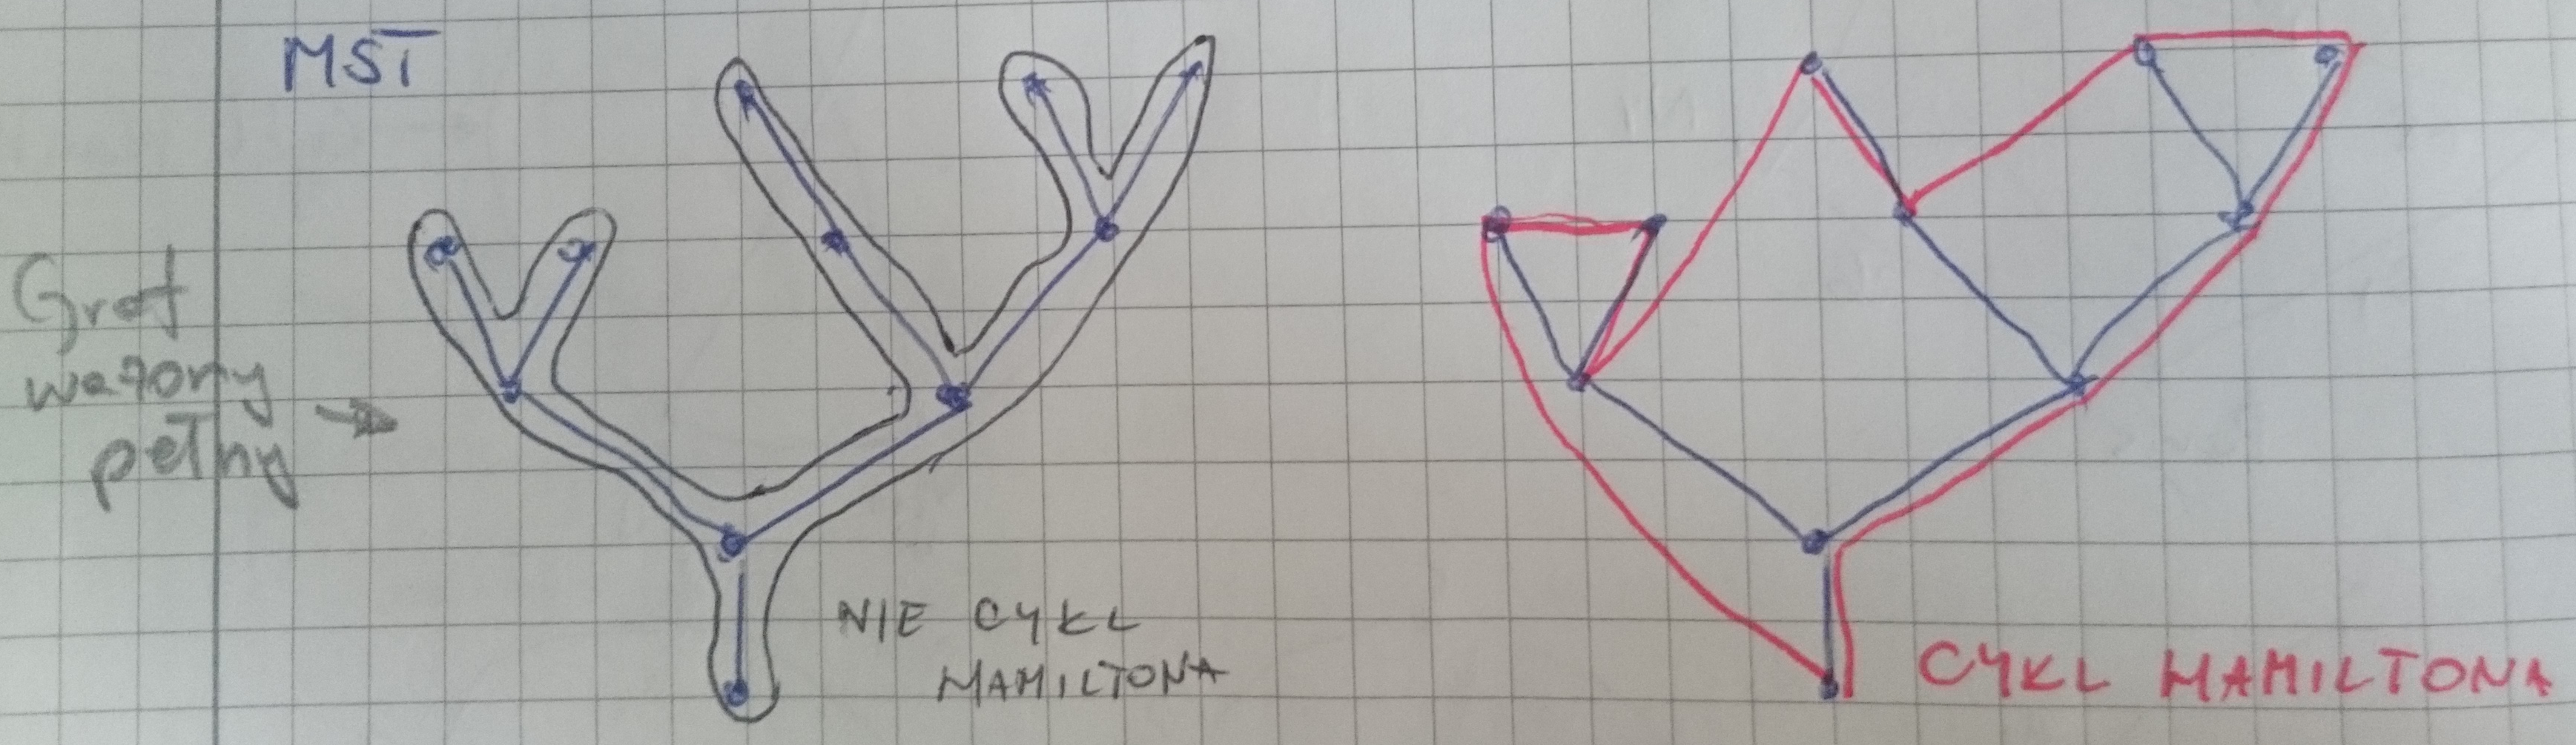
\includegraphics[width=.9\textwidth]{img/g8}
\end{figure}

%--------------------------------------------------
\end{document}
